\documentclass{article}
\usepackage{graphicx} % Required for inserting images
\usepackage[T1]{fontenc}
\usepackage[polish]{babel}
\usepackage[utf8]{inputenc}
\usepackage{amssymb}
\usepackage{tikz}
\usepackage{amsmath}
\usepackage{listings}
\usepackage{graphicx}
\usepackage[a4paper, left=40mm, right=40mm, top=30mm, bottom=30mm]{geometry}
\usepackage[indent=0pt]{parskip}

\graphicspath{ {./images/} }
\usepackage{csquotes}

\title{Indeksowa organizacja pliku - B-drzewo}
\author{Jerzy Szyjut}
\date{10.12.2024}

\begin{document}

\maketitle

\section{Wybór implementacji}
W ramach mojego projektu zaimplementowałem B-drzewo z wstawianiem i szukaniem rekordów (mechanizm kompensacji i dzielenia węzłów). Program zaimplementowałem w języku C++. 


\section{Wprowadzenie teoretyczne}
\subsection{Wstęp}

B-drzewo to zbalansowana struktura danych, wykorzystywana głównie w systemach baz danych i systemach plików, dzięki efektywnej obsłudze dużych zbiorów danych. Jest to drzewo wyszukiwań ogólnego przeznaczenia, które charakteryzuje się niską wysokością, co przekłada się na małą liczbę operacji dyskowych. Każdy węzeł w B-drzewie może mieć więcej niż dwóch potomków i przechowywać wiele kluczy.

Stałe używane w dalszej części dokumentu:
\begin{itemize}
    \item $d$ - minimalna liczba elementów w węźle
    \item $n$ - liczba kluczy w drzewie
    \item $h$ - wysokość drzewa
\end{itemize}

\subsection{Struktura B-drzewa}
B-drzewo spełnia następujące warunki:
\begin{itemize}
    \item Każdy węzeł (poza korzeniem) ma co najmniej $d$ kluczy.
    \item Każdy węzeł może mieć maksymalnie $2d$ kluczy.
    \item Każdy węzeł wewnętrzny posiada liczbę potomków równą liczbie kluczy + 1.
    \item Wszystkie liście znajdują się na tym samym poziomie.
    \item Klucze w węzłach są uporządkowane niemalejąco.
\end{itemize}

\begin{center}
Przykład B-drzewa o stopniu $d=2$ i $n=10$

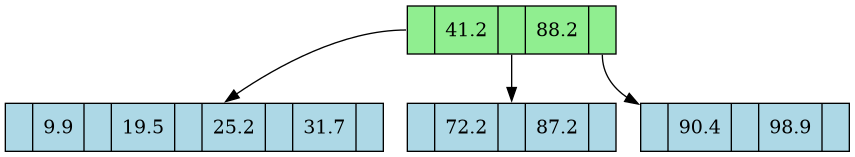
\includegraphics[width=0.8\textwidth]{images/bdrzewo-10.png}    
\end{center}

\section{Operacje na B-drzewach}
\subsection{Przeszukiwanie}
Przeszukiwanie w B-drzewie polega na porównywaniu klucza z wartościami w węzłach. Jeśli klucz jest w danym węźle, zwracamy go; jeśli nie, przechodzimy do odpowiedniego poddrzewa.

Złożoność czasowa wynosi $O(\log n)$, ponieważ B-drzewo jest zbalansowane, a liczba kluczy w węźle jest ograniczona.

\subsection{Wstawianie kluczy}
Operacja wstawiania odbywa się w następujących krokach:
\begin{enumerate}
    \item Znajdujemy liść, w którym klucz powinien się znaleźć.
    \item Jeśli węzeł liścia ma mniej niż $2d$ kluczy, wstawiamy klucz do węzła.
    \item Jeśli węzeł jest ma $2d$ klucz, a jeden z sąsiednich węzłów ma mniej niż $2d - 1$ kluczy, to rozdzielamy po równo klucze między węzeł i sąsiada (trzeba też uwzględnić, że możliwe że będziemy musieli zmienić klucz w rodzicu)
    \item Jeśli kompensacja jest możliwa, dzielimy go na dwa węzły, a środkowy klucz przenosimy do węzła nadrzędnego.
    \item W razie potrzeby proces podziału propaguje się do korzenia, co może zwiększyć wysokość drzewa.
\end{enumerate}

\section{Analiza złożoności}
\subsection{Złożoność operacji}
\begin{itemize}
    \item \textbf{Przeszukiwanie:} $O(\log n)$
    \item \textbf{Wstawianie:} $O(\log n)$ w przypadku potrzeby propagacji podziału.
\end{itemize}
\subsection{Wysokość drzewa}
Wysokość drzewa spełnia poniższy warunek
\begin{center}
    $log_{2d+1} (n+1) \le h \le log_{d+1} ((n+1)/2)+1$
\end{center}

\section{Opis implementacji przyjętej metody}
W swojej metodzie wczytuję pojedynczo węzły do pamięci operacyjnej programu, co pozwala na stałe zużycie pamięci niezależnie od ilości danych. Węzły zapisuję do pamięci masowej tylko, jeśli zostały zmodyfikowane. Jako, że korzeń jest bardzo często używanym węzłem, jest przechowywane cały czas w pamięci operacyjnej programu, w przypadku aktualizacji jest zapisywany w pamięci masowej.


\section{Specyfikacja formatu pliku}
Plik bdrzewa jest plikiem w którym zapisuję węzły b-drzewa. Każdy węzeł zajmuje tyle samo miejsca na dysku, niezależnie od tego ile liczb przechowuje. Dzięki temu czas odczytu węzła z dysku jest stały. Każdy węzeł składa się z:
\begin{itemize}
    \item Identyfikatora
    \item Identyfiaktora rodzica
    \item $d$ kluczy
    \item $d$ adresów
    \item $d+1$ wskaźników na klucze
\end{itemize}

\section{Sposób prezentacji wyników działania programu}
Menu wyboru akcji w programie jest wywoływane po każdej operacji. Menu na dodawanie nowych elementów ręcznie, za pomocą generatora liczb losowych, na wprowadzenie do programu sekwencji instrukcji, wyszukiwaniu elementów w b-drzewie po kluczu i wypisaniu licznika operacji.

\subsection{Menu}
\begin{lstlisting}
i - insert
r - insert random
s - search
p - print tree
d - toggle print after each action
c - print counters
f - execute instructions from file
q - quit
\end{lstlisting}

\subsection{Wyświetlanie reprezentacji B-drzewa}
Reprezentacja b-drzewa jest wyświetlana w formie graficznej przy pomocy biblioteki graphviz. Przykład poniżej.
\begin{center}
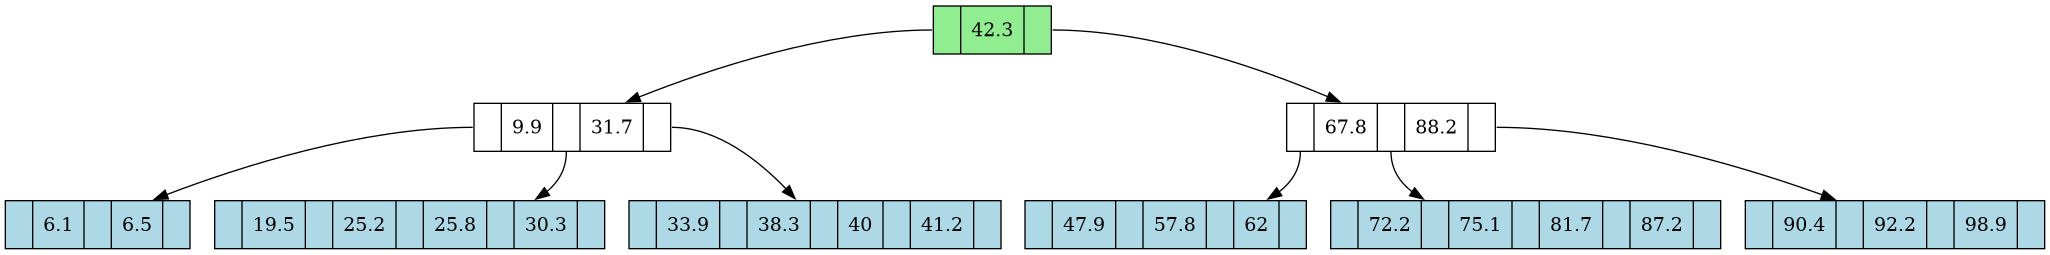
\includegraphics[width=1\textwidth]{images/bdrzewo-przyklad.png}    
\end{center}

\section{Eksperyment}
Przy pomocy programu przeprowadziłem eksperymenty losując liczby i wstawiając je do b-drzewa przy tym samym ziarnie generatora liczb losowych. Zrobiłem tak dla $d$ równemu 2, 10, 100, 1000.

\begin{center}
\begin{tabular}{|c|c|c c c| c |c c c|}
\hline
$d$ & $n$ & $r$ & $w$ & $r/w$ & $\alpha$ & min $h$ & max $h$ & $h$ \\
\hline
2 & 10 & 14 & 22 & 0.6364 & 0.625 & 1 & 2 & 2 \\
2 & 100 & 586 & 354 & 1.6554 & 0.7353 & 2 & 4 & 4 \\
2 & 1000 & 8549 & 4114 & 2.0780 & 0.7813 & 4 & 6 & 5 \\
2 & 10000 & 105231 & 42869 & 2.4547 & 0.7783 & 5 & 8 & 7 \\
2 & 100000 & 1211371 & 433473 & 2.7946 & 0.7752 & 7 & 10 & 8 \\
\hline
10 & 10 & 0 & 11 & 0 & 0.5 & 0 & 1 & 1 \\
10 & 100 & 130 & 139 & 0.9353 & 0.7143 & 1 & 2 & 2 \\
10 & 1000 & 3029 & 1846 & 1.6408 & 0.7463 & 2 & 3 & 3 \\
10 & 10000 & 42676 & 21442 & 1.9903 & 0.7808 & 3 & 4 & 4 \\
10 & 100000 & 484565 & 215829 & 2.2451 & 0.7708 & 3 & 5 & 5 \\
\hline
100 & 10 & 0 & 11 & 0 & 0.05 & 0 & 1 & 1 \\
100 & 100 & 0 & 101 & 0 & 0.5 & 0 & 1 & 1 \\
100 & 1000 & 918 & 1081 & 0.8492 & 0.5556 & 1 & 2 & 2 \\
100 & 10000 & 11585 & 11110 & 1.0428 & 0.7458 & 1 & 2 & 2 \\
100 & 100000 & 194824 & 114349 & 1.7038 & 0.7287 & 2 & 3 & 3 \\
\hline
1000 & 10 & 0 & 11 & 0 & 0.005 & 0 & 1 & 1 \\
1000 & 100 & 0 & 101 & 0 & 0.05 & 0 & 1 & 1 \\
1000 & 1000 & 0 & 1001 & 0 & 0.5 & 0 & 1 & 1 \\
1000 & 10000 & 8093 & 10060 & 0.8045 & 0.7139 & 1 & 2 & 2 \\
1000 & 100000 & 100462 & 101055 & 0.9941 & 0.7318 & 1 & 2 & 2 \\
1000 & 1000000 & 1024251 & 967807 & 1.0583 & 0.7309 & 1 & 2 & 2 \\
\hline
\end{tabular}

\begin{center}
    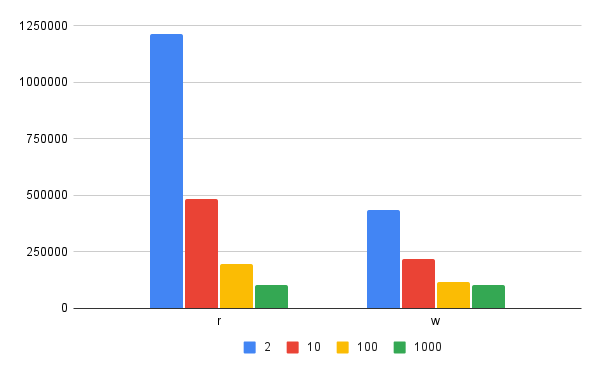
\includegraphics[width=0.8\textwidth]{images/chart.png}
    
    Liczba odczytów i zapisów zależnie od $d$ dla $n=100000$
    
    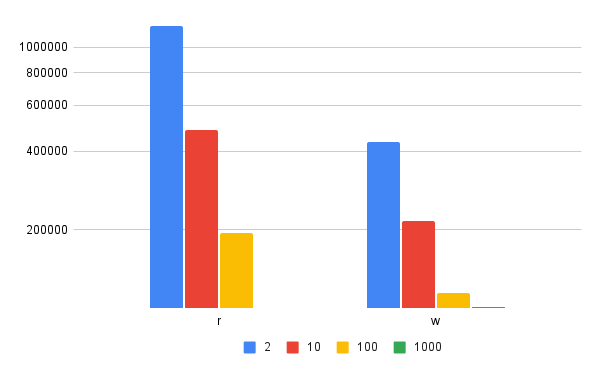
\includegraphics[width=0.8\textwidth]{images/chart_log.png}
    
    Liczba odczytów i zapisów zależnie od $d$ dla $n=100000$, oś Y w skali logarytmicznej
\end{center}

\end{center}


\section{Wnioski}
B-drzewo to wydajna struktura indeksowa, która zapewnia niską wysokość drzewa nawet przy dużych zbiorach danych, co pozwala na szybkie operacje wstawiania i wyszukiwania. Eksperymenty wykazały, że wraz ze wzrostem stopnia drzewa $d$, zmniejsza się jego wysokość, co poprawia wydajność operacji kosztem większego rozmiaru węzłów. Wartość współczynnika $\alpha$, oscylująca między 0.7 a 0.8, zapewnia bardzo dobre wykorzystanie przestrzeni. Dla dużych danych lepsze są wyższe wartości $d$, ponieważ drzewo pozostaje niemal płaskie, co znacznie redukuje liczbę operacji zapisu i odczytu. Wartość $d$ powinna być niższa od wartości $n$, aby współczynnik $\alpha$ był wysoki. Poza tym im wyższa wartość $d$ tym mniejsza ilość operacji zapisu i odczytu do pliku. Jednak dla dużych wartości $d$ algorytm może być wolniejszy, jako że w każdym węźle musi przeszukiwać więcej wartości. 

\end{document}
